\documentclass[a4paper]{article}
\usepackage{url} 
\usepackage{geometry}
\usepackage{graphicx}
\usepackage[parfill]{parskip}
\usepackage{pgfplots}
\usetikzlibrary{external}
\tikzset{external/system call={lualatex \tikzexternalcheckshellescape 
         -enable-write18 -halt-on-error -interaction=nonstopmode 
         -jobname "\image" "\texsource"}}
\tikzexternalize % activate!
\begin{document}
\begin{figure}[ht]
 
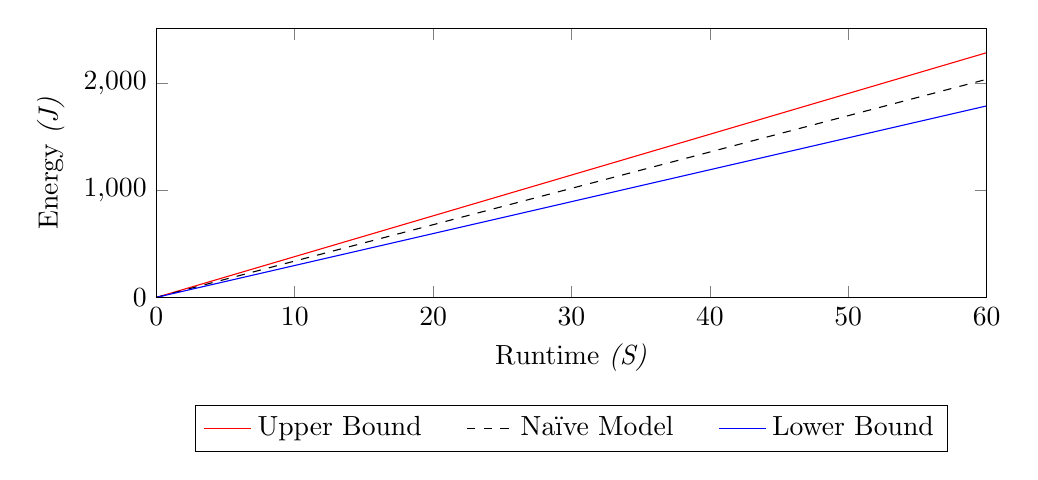
\begin{tikzpicture}
  \begin{axis}[no markers, ylabel={Energy \emph{(J)}}, xlabel={Runtime \emph{(S)}}, axis on top,
    ymin=0,
    xmin=0, xmax=60,
    width=\textwidth,
    height=5cm,
    legend style={at={(0.5,-0.4)}, anchor=north,legend columns=-1, /tikz/every even column/.append style={column sep=0.5cm}}
    ]
     \pgfmathsetmacro{\baseline}{29.857}
     \pgfmathsetmacro{\power}{38.157}
     \pgfmathsetmacro{\seconds}{40}
     \pgfmathsetmacro{\energy}{\power * \seconds}
     \pgfmathsetmacro{\baselineenergy}{\baseline * \seconds}

     \addplot[domain=0:60, red] {\power * x};
     \addplot[domain=0:60, dashed] {(\power + \baseline) * 0.5 * x};
     \addplot[domain=0:60, blue] {\baseline * x};

     \addlegendentry{Upper Bound}
     \addlegendentry{Na\"{\i}ve Model}
     \addlegendentry{Lower Bound}
  \end{axis}
\end{tikzpicture}
\end{figure}
\end{document}
